\svnInfo $Id$
% --------------------------------------------------------------------------------
\chapter{Grid geometry}
% --------------------------------------------------------------------------------


% --------------------------------------------------------------------------------
\section{Horizontal grid}
% --------------------------------------------------------------------------------

The horizontal ICON grid consists of a set of spherical triangles that seamlessly span the entire sphere. The grid is constructed from an icosahedron (see Figure 
\ref{fig_ico_a}) which is projected onto a sphere. The spherical icosahedron (Figure \ref{fig_ico_b}) consists of $20$ equilateral spherical triangles. The edges of each triangle 
are bisected into equal halves or more generally into $n$ equal sections. Connecting the new edge points by great circle arcs yields $4$ or more generally $n^2$ spherical triangles 
within the original triangle (Figure \ref{fig_bisect}, \ref{fig_nsect}). 

\begin{figure}[h]
  \begin{minipage}[b]{0.4\textwidth}
    \centering
    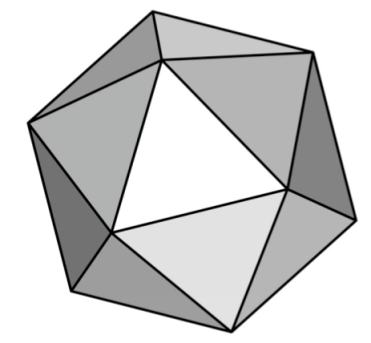
\includegraphics[width=0.69\textwidth]{icosahedron.png}
    \subcaption{}\label{fig_ico_a}
  \end{minipage}\hfill
  \begin{minipage}[b]{0.4\textwidth}
    \centering
    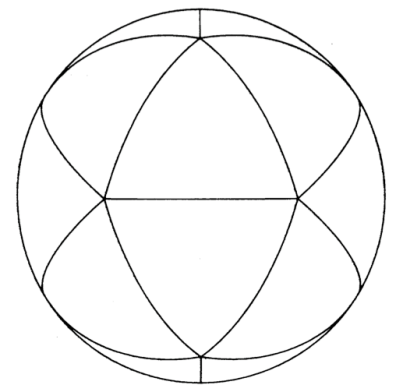
\includegraphics[width=0.69\textwidth]{icosahedron_spherical.png}
    \subcaption{}\label{fig_ico_b}
  \end{minipage}\hfill
  \caption{Icosahedron before (a) and after (b) projection onto a sphere }

\hfill

  \begin{minipage}[b]{0.4\textwidth}
    \centering
    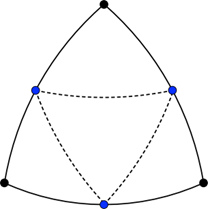
\includegraphics[width=0.69\textwidth]{bisection.png}
    \subcaption{}\label{fig_bisect}
  \end{minipage}\hfill
  \begin{minipage}[b]{0.4\textwidth}
    \centering
    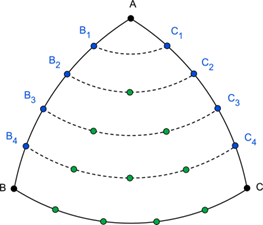
\includegraphics[width=0.78\textwidth]{nsection.png}
    \subcaption{}\label{fig_nsect}
  \end{minipage}\hfill
  \caption{(a) Bisection of the original triangle edges (b) More general division into $n$ equal sections}
\end{figure}

ICON grids are constructed by an initial root division into $n$ sections (\textbf{R}n) followed by $k$ bisection steps (\textbf{B}k), 
resulting in a \textbf{R}n\textbf{B}k grid. Figures \ref{fig_R2B00} and \ref{fig_R2B02} show \textbf{R}2\textbf{B}00 and 
\textbf{R}2\textbf{B}02 ICON grids. Such grids avoid polar singularities of latitude-longitude grids (Figure \ref{fig_lonlat}) 
and allow a high uniformity in resolution over the whole sphere.

\begin{figure}[h]
  \begin{minipage}[b]{0.3\textwidth}
    \centering
    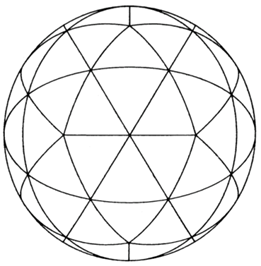
\includegraphics[width=0.9\textwidth]{icon_grid_R2B00.png}
    \subcaption{}\label{fig_R2B00}
  \end{minipage}\hfill
  \begin{minipage}[b]{0.3\textwidth}
    \centering
    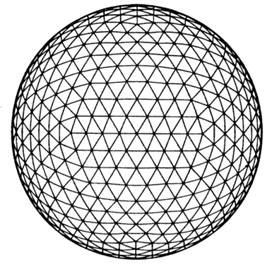
\includegraphics[width=0.95\textwidth]{icon_grid_R2B02.png}
    \subcaption{}\label{fig_R2B02}
  \end{minipage}\hfill
  \begin{minipage}[b]{0.3\textwidth}
    \centering
    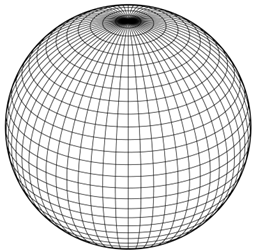
\includegraphics[width=0.95\textwidth]{lon-lat-grid.png}
    \subcaption{}\label{fig_lonlat}
  \end{minipage}\hfill
  \caption{(a) R2B00 grid. (b) R2B02 grid. (c) traditional regular latitude-longitude grid with polar singularities}
\end{figure}

Throughout this document, the grid is referred to as the ``\textbf{R}n\textbf{B}k grid'' or ``\textbf{R}n\textbf{B}k resolution''. For a given resolution \textbf{R}n\textbf{B}k, 
the total number of cells, edges, and vertices can be computed from
\begin{eqnarray*}
 n_{c} &=& 20\,n^{2}\,4^{k} \\
 n_{e} &=& 30\,n^{2}\,4^{k} \\
 n_{v} &=& 10\,n^{2}\,4^{k} + 2
\end{eqnarray*}
The average cell area $\overline{\Delta A}$ can be computed from
\begin{align*}
 \overline{\Delta A} = \frac{4\pi\,r_{e}^{2}}{n_{c}}\,,
\end{align*}
with the earth radius $r_{e}$, and $n_{c}$ the total number of cells. Based on $\overline{\Delta A}$ one can derive an estimate of the average grid resolution 
$\overline{\Delta x}$:
\begin{align*}
 \overline{\Delta x} = \sqrt{\overline{\Delta A}} = \sqrt{\frac{\pi}{5}} \frac{r_{e}}{n\,2^{k}}
\end{align*}
Visually speaking, $\overline{\Delta x}$ is the edge length of a square which has the same area as our triangular cell.


In Table \ref{tab_res}, some characteristics of frequently used ICON grids are given. The table contains information about the total number of triangles ($n_{c}$), the average 
resolution $\overline{\Delta x}$, and the maximum/minimum cell area. The latter may be interpreted as the area for which the prognosed meteorological quantities (like temperature, 
pressure, \dots) are representative. Some additional information about ICON's horizontal grid can be found in \citet{Wan13}.

\begin{table}[H]
  \caption{Characteristics of frequently used ICON grids. $\Delta A_{max}$ and $\Delta A_{min}$ refer to the maximum and minimum area of the grid cells, respectively.}\label{tab_res}
  \begin{center}
    \begin{tabular}{p{2.0cm}>{\raggedleft\arraybackslash}p{3.5cm}>{\centering\arraybackslash}p{3.5cm}>{\raggedleft\arraybackslash}p{2.5cm}>{\raggedleft\arraybackslash}p{2.5cm}}
    \toprule
    \textbf{Grid} & \textbf{number of cells ($n_{c}$)} & \textbf{avg.\ resolution [km]} & $\mathbf{\Delta A_{max}\,[km^{2}]}$ & $\mathbf{\Delta A_{min}\,[km^{2}]}$\\
    \midrule
    R2B04         &    20480                           &  157.8                         &  25974.2                  &  18777.3 \\
    R2B05         &    81920                           &   78.9                         &  6480.8                   & 4507.5\\
    R2B06         &   327680                           &   39.5                         &  1618.4                   & 1089.6 \\
    R2B07         &  1310720                           &   19.7                         &  404.4                    & 265.1 \\
    R3B07         &  2949120                           &   13.2                         &  179.7                    & 116.3 \\
    \bottomrule
    \end{tabular}
  \end{center}
\end{table}

\begin{note}
  \textbf{\textcolor{red}{The first operational version of ICON is
      based on the R3B07 grid, thus, having a horizontal resolution of
      about $13\,\mathrm{km}$!}}
\end{note}


% --------------------------------------------------------------------------------
\section{Vertical grid}
% --------------------------------------------------------------------------------

The vertical grid consists of a set of vertical layers with height-based vertical coordinates.
Each of these layers carries the horizontal $2D$ grid structure, thus forming the $3D$ structure of the grid.
The ICON grid employs a Lorenz-type staggering with the vertical velocity defined at the boundaries of layers (half levels) 
and the other prognostic variables in the center of the layer (full levels).

To improve simulations of flow past complex topography, the ICON model employs a smooth level vertical (SLEVE) coordinate~\citep{Leuenberger2010}. 
It allows for a faster transition to smooth levels in the upper troposphere and lower stratosphere, as compared to the classical height-based Gal-Chen 
coordinate. In the operational setup, the transition from terrain following levels in the lower atmosphere to constant height levels is completed 
at $z=16\,\mathrm{km}$. Model levels above are flat. The required smooth large-scale contribution of the model topography is generated by 
digital filtering with a $\nabla^2$-diffusion operator. Figure~\ref{fig:vertical_levels} shows the (half) levels of the operational 
ICON setup with 90 vertical levels. The table to the right shows the height above ground of selected half levels (for zero height topography) 
and the corresponding pressure, assuming the US standard atmosphere. Standard heights for all $91$ half levels are given in Table 
\ref{tab:half_level_heights}.

\textbf{Please note that for grid cells with non-zero topography these values only represent rough estimates of the true level height. 
Actual heights and layer thicknesses may vary considerably from location to location, due to grid level stretching/compression over 
non-zero topography.}
  
%In the operational setup, the transition from terrain following levels in the lower atmosphere to constant height levels is completed at 
%$z=16\,\mathrm{km}$. Model levels above are flat.



% ---------------------------------------------------------------------------------------
% ICON vertical levels -- SLEVE coordinates
% 
% author: 07/2013: F. Prill, DWD
% created with a Matlab script and the following settings:
%
%   min_lay_thckn   = 20.;        % Layer thickness of lowermost layer
%   top_height      = 75000.;     % Height of model top
%   stretch_fac     = 0.9;        % Scaling factor for stretching/squeezing 
%                                 % the model layer distribution
%   
%   decay_scale_1   = 4000.;      % Decay scale of large-scale topography component
%   decay_scale_2   = 2500.;      % Decay scale of small-scale topography component
%   decay_exp       = 1.2;        % Exponent for decay function
%   flat_height     = 16000.;     % Height above which the coordinate surfaces are flat
%   topo            = 0.;
%   topo_smt        = 0.;  
% 
% see also ICON routines "init_sleve_coord", "init_vert_coord"        
%
% Input files for this figure are created with the following commands:
%
%  octave -q --eval 'nlev=90; [z_m, z_i, pres_m, pres_i] = icon_levels(nlev); printf("k z p\n"); for k=1:nlev printf("%d %5.3f %5.3f\n",k,z_i(k),z_i(k)-z_i(k+1));end' > vertical_levels_i.txt 
%
%  octave -q --eval 'nlev=90; [z_m, z_i, pres_m, pres_i] = icon_levels(nlev); printf("k z p\n"); for k=[1:5:nlev,nlev] printf("%d %d %5.1f\n",k,z_i(k),pres_i(k));end' > vertical_levels_i_small.txt 
%
% (Alternatively, for a pressure plot:)
%  octave -q --eval 'nlev=90; [z_m, z_i, pres_m, pres_i] = icon_levels(nlev); printf("k z p\n"); for k=1:nlev printf("%d %5.3f %5.3f\n",k,z_i(k),pres_i(k));end' > vertical_levels_i.txt 
%
%
% ---------------------------------------------------------------------------------------
\begin{figure}[hbt]
\begin{tabbing}
  \begin{minipage}[t]{0.65\linewidth} \vspace*{0pt}%
    \pgfplotstableread{level_tables/vertical_levels_i.txt}{\loadedtable}
    \pgfplotsset{
      tick label style={font=\small},
    }
  \begin{tikzpicture}[scale=0.7, transform shape]
    \begin{axis}[ minor tick num=1, axis x line=bottom, axis y line=left, 
                  every inner x axis line/.append style= {|->},
                  every inner y axis line/.append style= {|->}, 
                  width=10cm,height=14.5cm, ymajorgrids,
                  xlabel=level, 
                  scaled y ticks = false,
                  ylabel=\textbf{\color{blue}$z~\text{[m]}$}, enlargelimits=false,
                  every axis y label/.style={at={(current axis.north west)},
                                             yshift=3em,anchor=north east}
                ]
      \addplot[blue,mark=*] table[x={k},y={z}] \loadedtable;
    \end{axis}
    \begin{axis}[ minor tick num=1, axis x line=bottom, axis y line=right, 
                  every inner x axis line/.append style= {|->},
                  every inner y axis line/.append style= {|->}, 
                  width=10cm,height=14.5cm, 
                  scaled y ticks = false,
                  ylabel=\textbf{\color{red}$\Delta z~\text{[m]}$}, enlargelimits=false ,
                  every axis y label/.style={at={(current axis.north east)},
                                             yshift=3em,anchor=north west}
                 ]
      \addplot[red,only marks,mark=diamond] table[x={k},y={p}] \loadedtable;
    \end{axis}
  \end{tikzpicture}
  \end{minipage}
%
%
\=
%
%
  \begin{minipage}[t]{0.35\linewidth}\vspace*{0em}%
   \renewcommand{\baselinestretch}{0.95}\normalsize%
   \pgfkeys{/pgf/number format/set thousands separator={\,}}
   \pgfplotstableread{level_tables/vertical_levels_i_small.txt}{\loadedtablesmall}\vspace*{0pt}%
   \pgfplotstabletypeset[ columns={k,z,p},every  head row/.style={after row={\hline}},
          font=\footnotesize,
          columns/k/.style={column name=$level$, column type=r,column type/.add={>{\columncolor[gray]{.8}}}{}},
          columns/z/.style={column name=$[m]$,   fixed,dec sep align},
          columns/p/.style={column name=$[Pa]$, fixed,dec sep align, zerofill,precision=1},
                        ] {\loadedtablesmall}
    \vspace*{1em}%
  \end{minipage}
\end{tabbing}
%
  \caption{Vertical half levels (blue) and layer thickness (red) of the ICON operational setup.
    The table of selected pressure values (for zero height) is based on the 1976 US standard atmosphere.}
  \label{fig:vertical_levels}%
\end{figure}


% --------------------------------------------------------------------------------
\section{Refined subregion over Europe (``local nest'')}
% --------------------------------------------------------------------------------

ICON has the capability for running global simulations with refined
domains (so called \emph{nests}).
%
The triangular mesh of the refined area is generated by bisection of
triangles in the global ``parent'' grid, see
Fig.~\ref{fig:icon_grid_refinement_zoom_view}.
In the vertical the global grid extends into the mesosphere (which
greatly facilitates the assimilation of satellite data) whereas the
nested domains extend only into the lower stratosphere in order to
save computing time. For the same orography the heights of levels $1$--$60$ of
the Europe nest are the same as those of levels $31$--$90$ of the global grid. 
In practice, however, near surface level heights of nests and the global 
domain differ due to the fact that the underlying orography differs, 
with deeper slopes and higher summits in the high resolution nests.

For each nesting level, the time step is automatically divided by a
factor of two.
%
Note that the grid nests are computed in a concurrent fashion:  
\begin{itemize}
\item Points that are covered by the refined subdomain additionally
  contain data for the global grid state.
\item The data points on the triangular grid are the cell
  circumcenters. Therefore the global grid data points are closely
  located to nest data sites, but they \emph{do not coincide} exactly 
  (see Fig.~\ref{fig:icon_grid_refinement_zoom_view}).
\end{itemize}


\begin{figure}[hbt]
  \centering
  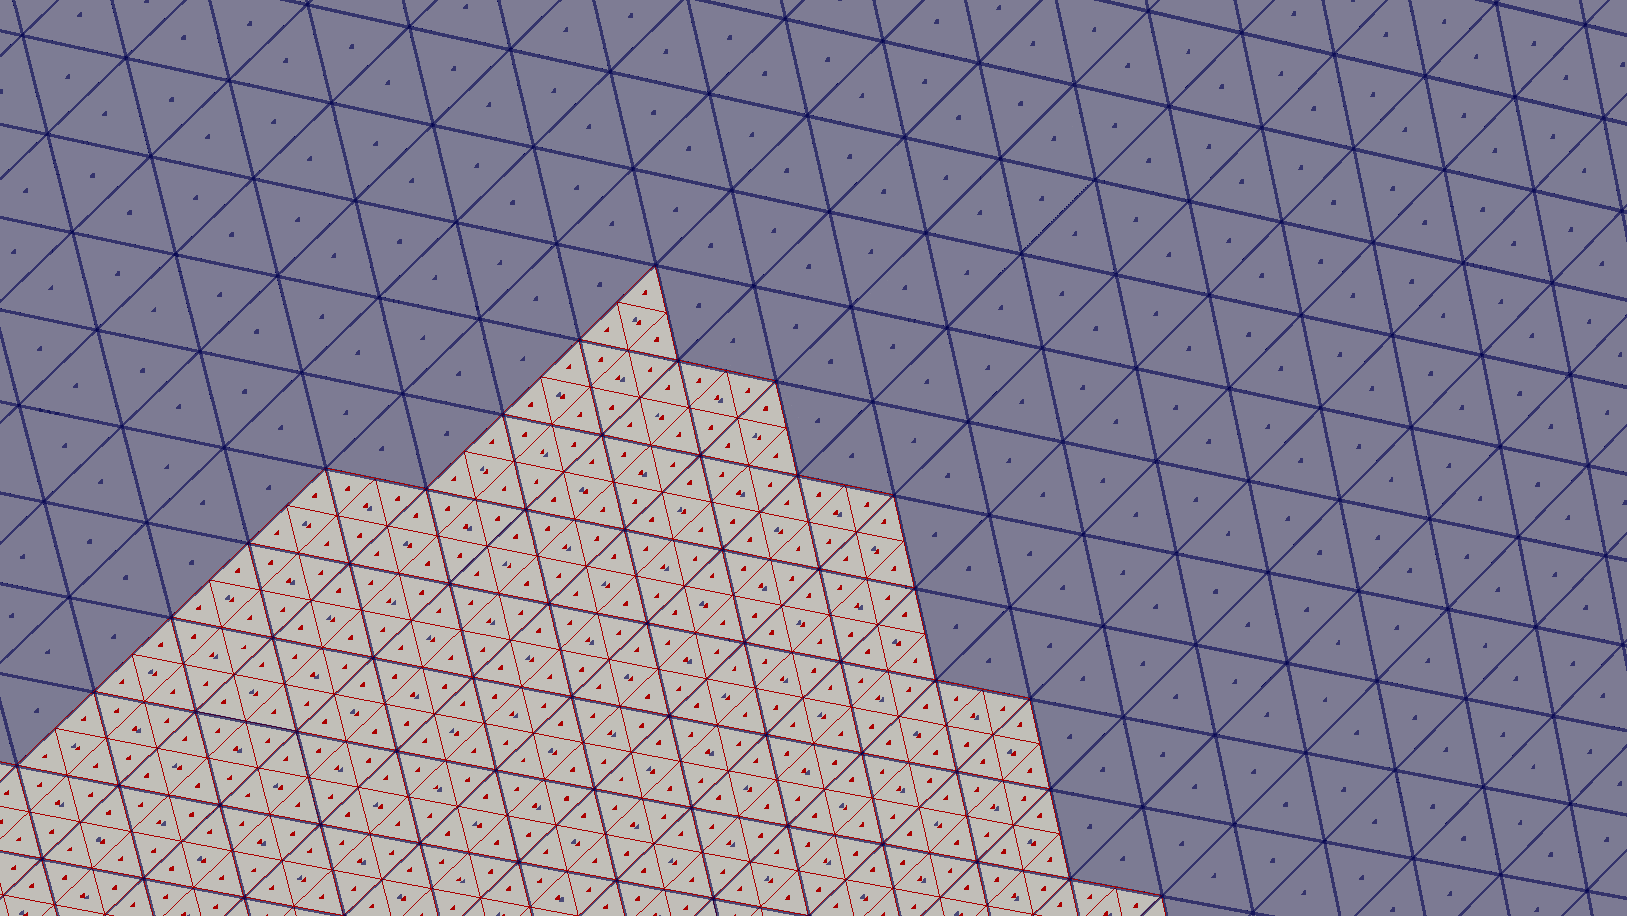
\includegraphics[width=0.90\textwidth]{pics/grid_refinement.png}
  \caption{ICON grid refinement (zoom view). Blue and red dots indicate the cell circumcenters for the global (``parent'') and the refined (``child'') domain, respectively.}
  \label{fig:icon_grid_refinement_zoom_view}
\end{figure}

ICON's refined subregion over Europe is comparable to the COSMO-EU region 
of DWD's COSMO model. Key figures like edge coordinates and mesh size of the COSMO-EU region and the ICON-EU nest 
are given in Table ~\ref{tab:COSMO_ICON_nest_extent}. The geographical location of the nest is visualized in 
Fig.~\ref{fig:EU_nest} and Fig.~\ref{fig:EU_nest_polar}.

\begin{table}
\centering
\caption{Key figures of the ICON-EU nest and the COSMO-EU region.}\label{tab:COSMO_ICON_nest_extent}
\begin{tabular}{|p{5cm}|l|l|}\hline
\rowcolor{Gray}
                           &    {\centering\textbf{ICON-EU nest}}                 &     {\centering\textbf{COSMO-EU}} \\ \hline\hline
% ----------------------------------------------------------------------------------------------------------------------------------------
geogr. coordinates         &    $23.5^\degree~\text{W}$ -- $62.5^\degree~\text{E}$    &     $\lambda_{\text{N}} = 170^\degree~\text{W}$, 
                                                                                          $\phi_{\text{N}}    =  40^\degree~\text{N}$,     \\
                           &    $29.5^\degree~\text{N}$ -- $70.5^\degree~\text{N}$   &      $18.0^\degree~\text{W} - 23.5^\degree~\text{E}$ \\
                           &                                                      &     $20.0^\degree~\text{S} - 21.0^\degree~\text{N}$  \\[0.5em]
mesh size                  &    $\approx 6.5~\km$ (R3B8)                          &     $0.0625^\degree$ ($\approx 7~\km$) \\
                           &    659156~triangles                                  &     $665 \times 657 = 436905$ grid points \\
vertical levels            &    60 levels                                         &     40 levels      \\
upper boundary             &    $22.5~\km$                                        &     $22.5~\km$ \\ \hline

\end{tabular}
\end{table}

\begin{note}
    \textbf{A test version of model simulations including the nesting region over
      Europe is running regularly, starting from 
      \begin{center}
        2015-03-26, 12~UTC (\texttt{para1}).
      \end{center}
      Currently only main forecasts at 00 and 12~UTC are performed, reaching out to 
      $120\,\mathrm{h}$, while forecasts starting at 06 and 18~UTC are limited 
      to $33\,\mathrm{h}$.
      }
\end{note}


Simulation on the global grid and the regional (Europe) domain are tightly coupled
(\emph{two-way nesting}):
Boundary data for the nest area is updated every time step (120~s).
%
Feedback of atmospheric prognostic variables (except precipitation) is
computed via relaxation on a 3~h time scale.

  
\begin{figure}[h]
  \begin{minipage}[b]{\textwidth}
    \centering
    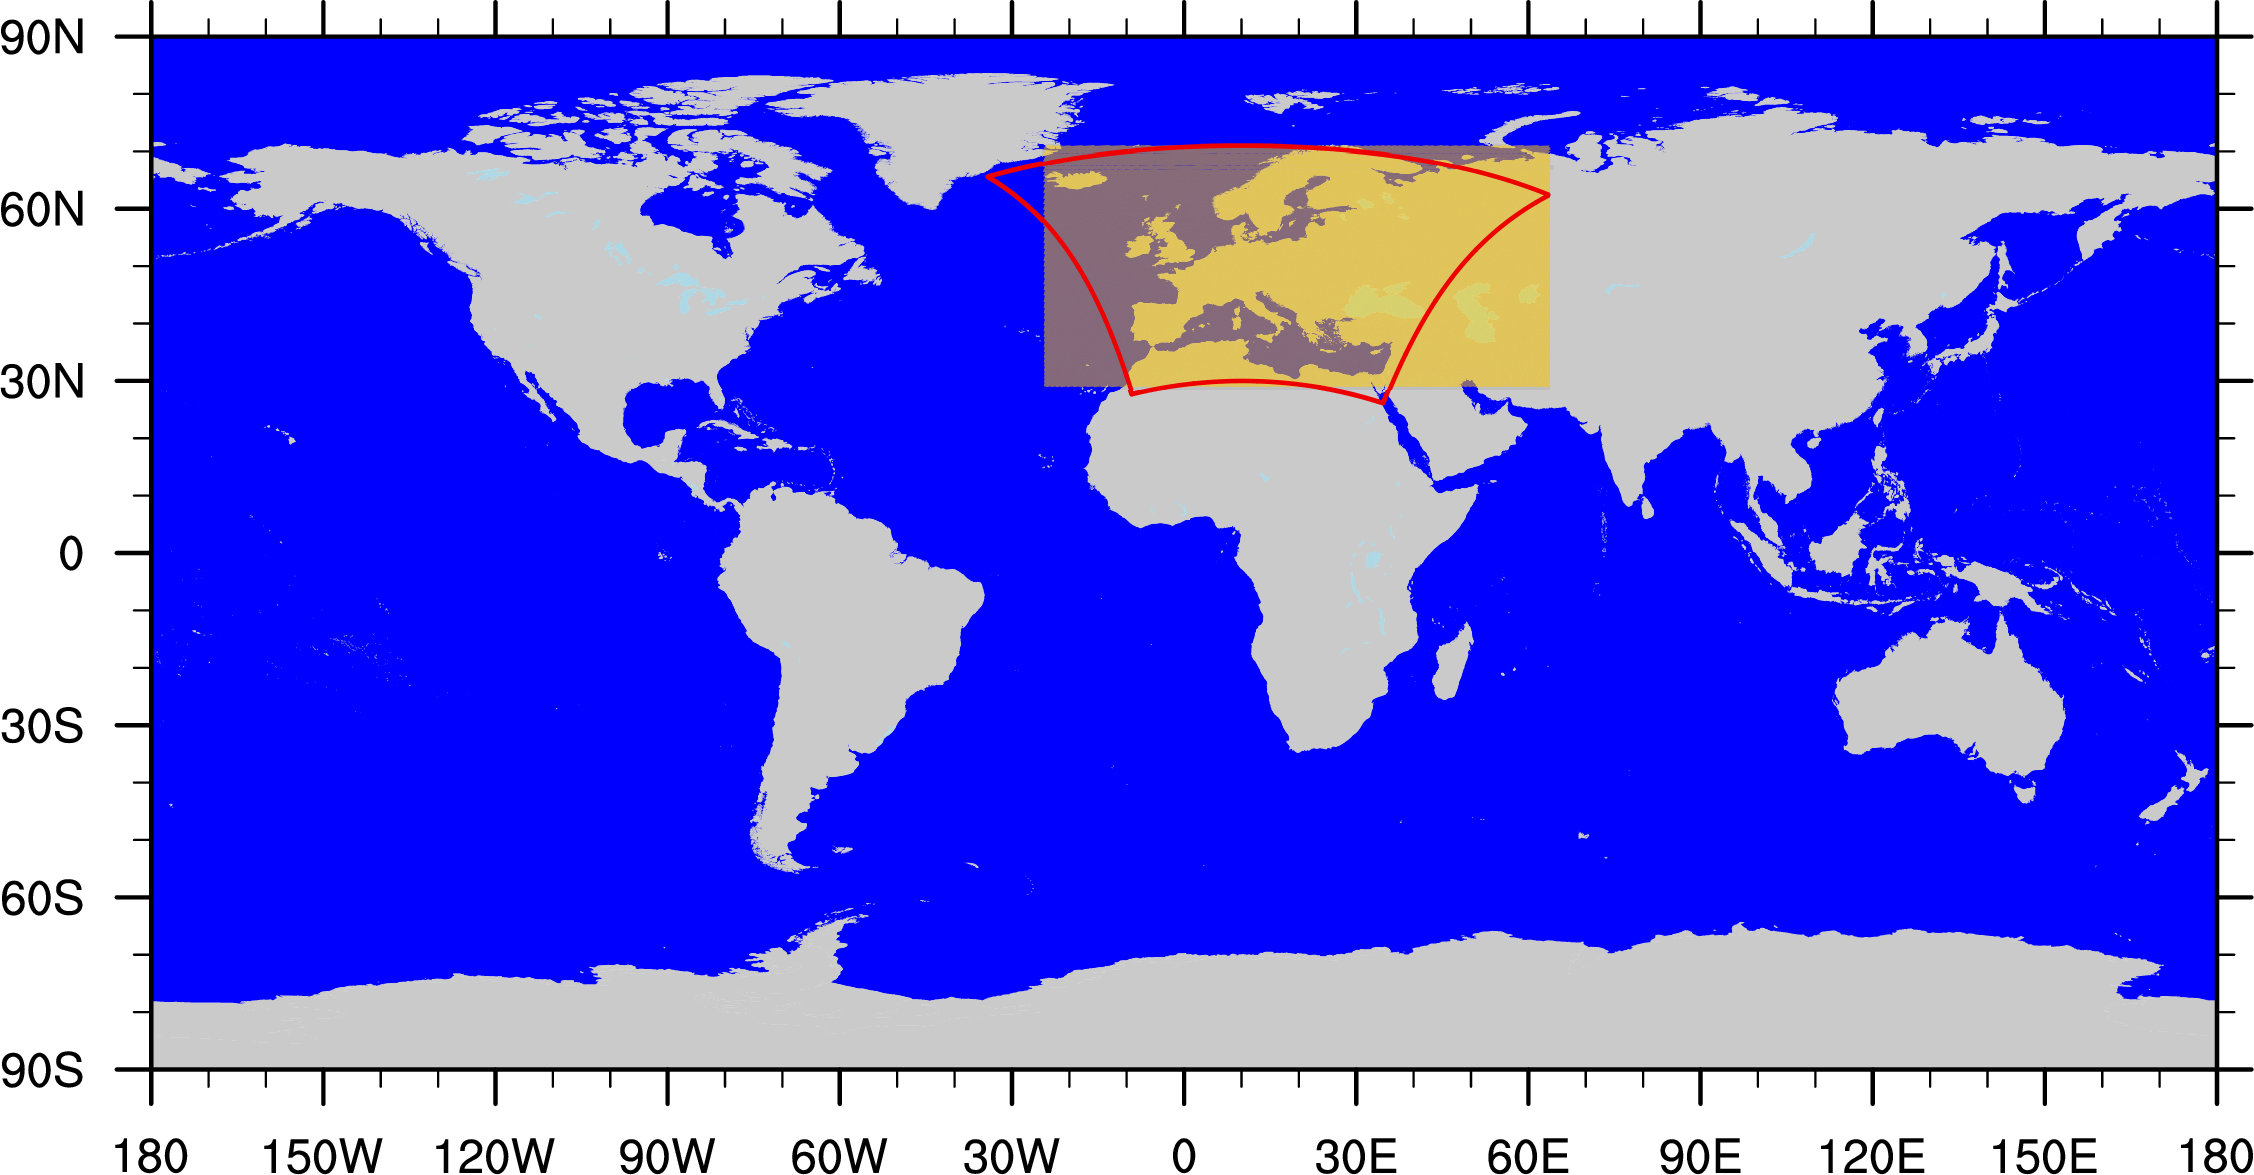
\includegraphics[width=0.90\textwidth]{ICON_EU_nest_1.png}
    \subcaption{}\label{fig:EU_nest}
  \end{minipage}
  \hfill
  \par
  \begin{minipage}[b]{\textwidth}
    \centering
    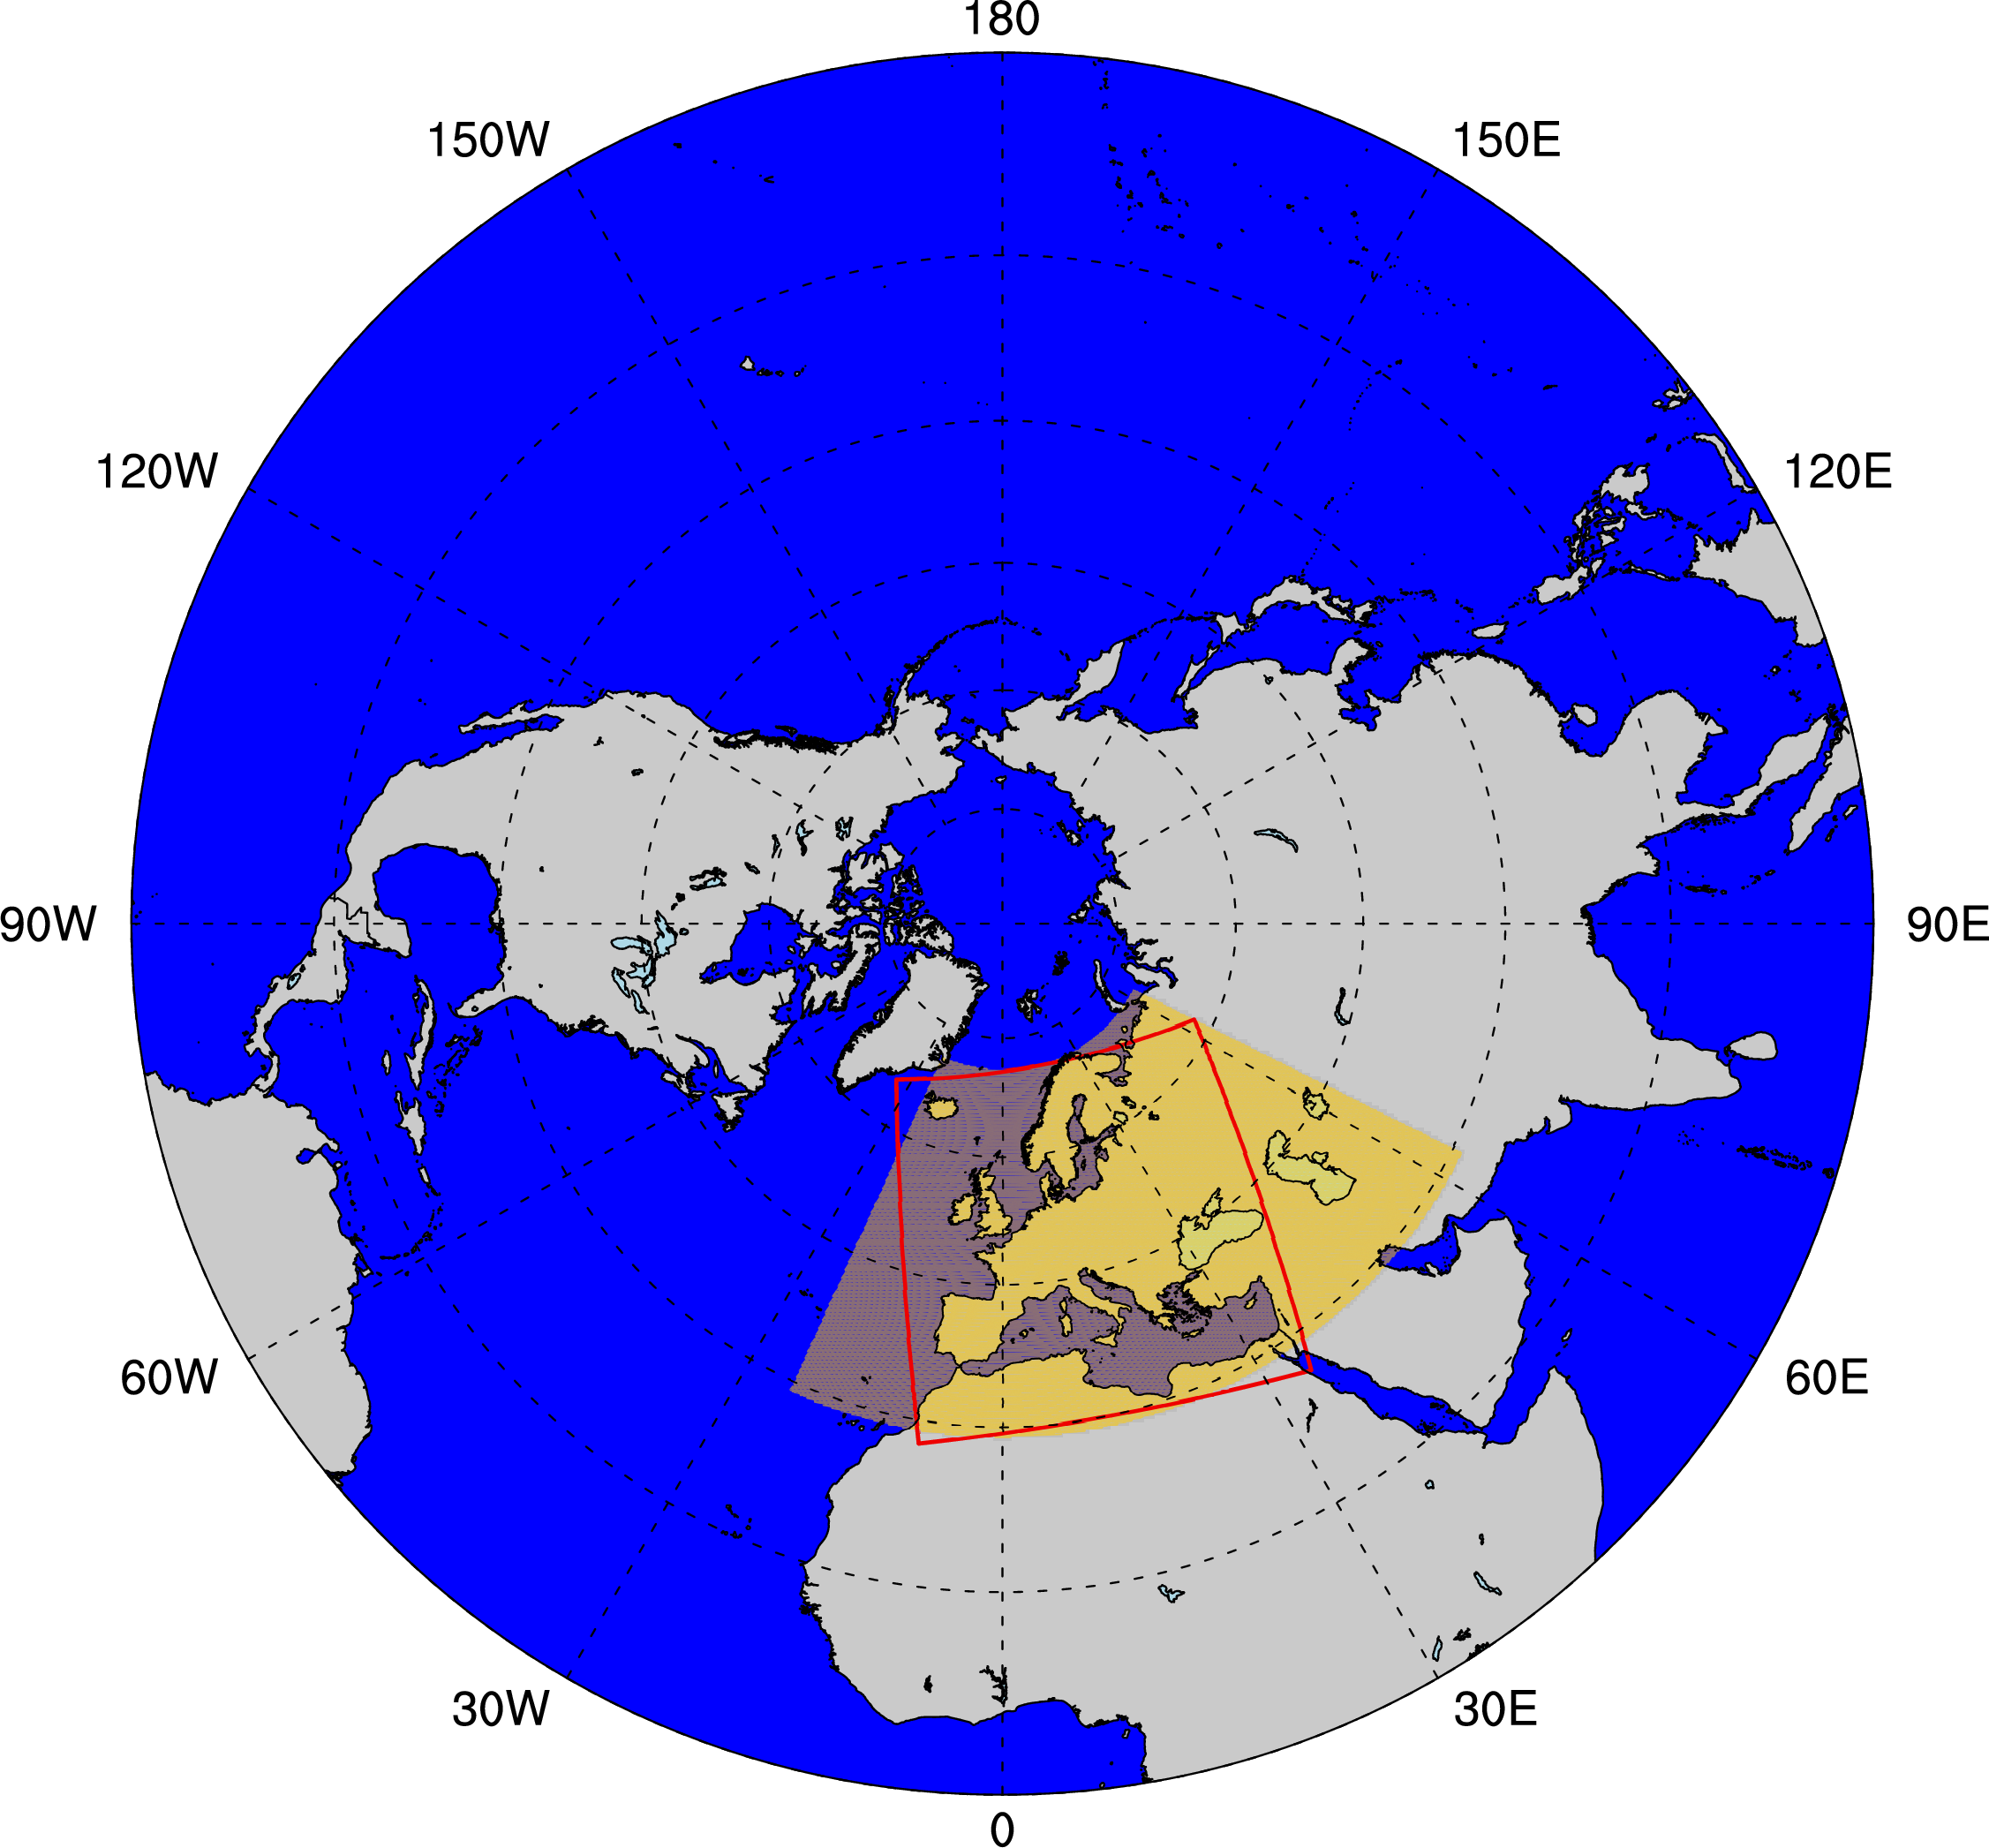
\includegraphics[width=0.80\textwidth]{ICON_EU_nest_2.png}
    \subcaption{}\label{fig:EU_nest_polar}
  \end{minipage}\hfill
  \caption{\ref{fig:EU_nest}: Horizontal extent of the ICON-EU nest
    (orange shaded area) in a cylindrical equidistant projection. For
    comparison, the outline of the COSMO-EU region is shown in red.
    \ref{fig:EU_nest_polar}:  Same as \ref{fig:EU_nest} but in a polar
    stereographic projection.}
\end{figure}




